\documentclass[11pt]{report}
\usepackage[utf8]{inputenc}
\usepackage{mathptm}
\usepackage{newcent}
\usepackage{xfrac}
\usepackage[letterpaper,left=1.1in,right=1.1in,top=1.1in,bottom=1.25in]{geometry}
\linespread{1.1}
\usepackage[perpage,symbol]{footmisc}
\usepackage{graphicx}
\usepackage{footnote}
\usepackage[margin=0pt,font=small,labelfont=bf]{caption}
\makesavenoteenv{tabular}
\def\topfraction{.9}
\def\bottomfraction{.9}
\def\textfraction{.1}
\def\floatpagefraction{.9}
\def\keystroke#1{$\left[\right.\!${\tt\bfseries #1}$\!\left.\right]$}
\def\key#1{\keystroke{#1}}
\def\keycombo#1#2{\keystroke{#1}\keystroke{#2}}
\def\keycontrol#1{\keycombo{Ctrl}{#1}}
\def\keyshift#1{\keycombo{Shift}{#1}}
\def\controlshift#1{\keystroke{Ctrl}\keystroke{Shift}\keystroke{#1}}
\def\keyctrlhat{\keycontrol{\char94}}
\def\keyhat{``{\tt\char94}''}
\def\keyctrlbackslash{\keycontrol{\char92}}
\def\keyctrlunderscore{\keycontrol{\char95}}
\def\keyunderscore{``{\tt\char95}''}
\def\terminal#1{{\tt#1}}
\def\icon#1{\raise-2pt\hbox{\includegraphics[height=11pt]{icons/#1.png}}}
\begin{document}
\thispagestyle{empty}
\begin{centering}
  {\Huge ELN}
  \vskip30pt

  {\Large an Electronic Lab Notebook}
  \vskip60pt

 
  {\large By Daniel A. Wagenaar}
  \vfill  

{\large version {\input{../src/version}}} 
\vskip10pt
  
  
  {Copyright (c) 2013--2020}
  
\end{centering}
\pagebreak
~
\vfill
\noindent Copyright (C) 2013--2020 Daniel A. Wagenaar\medskip

ELN is free software: you can redistribute it and/or modify
it under the terms of the GNU General Public License as published by
the Free Software Foundation, either version 3 of the License, or
(at your option) any later version.

This program is distributed in the hope that it will be useful,
but WITHOUT ANY WARRANTY; without even the implied warranty of
MERCHANTABILITY or FITNESS FOR A PARTICULAR PURPOSE.  See the
GNU General Public License for more details.

You should have received a copy of the GNU General Public License
along with this program.  If not, see http://www.gnu.org/licenses.
\pagebreak

\chapter{Introduction}

This document describes the installation and usage of ELN, an
electronic lab notebook written by Daniel Wagenaar.  This introduction
will not cover why you should keep a lab notebook, nor why an
electronic lab notebook may be desirable. You already know that.  It
will however, cover some of the ideas behind this particular
implementation.

\section{Why use ELN?}

There are any
number of software packages available that implement electronic
notebooks. So why should you choose ELN? ELN is for you if:
\begin{itemize}
  \item You want your notes to be stored in a human-readable format.
  \item You want your notes to be stored in a format that will be easy to
    parse electronically even 500 years from now.
  \item You want your notes to be protected against accidental
    deletion.
  \item You want your notes to be automatically dated.
  \item You want to concentrate on entering text and not on
    formatting.
  \item You want to be able to include images and simple graphics with
    your notes and you want that to be easy.
  \item You want your notebook software to be fast, even with thousands
    of pages of notes.
  \item You like your software to be open-source so that you can make
    your own improvements to it, and be confident that you can still
    run it 20 years from now.
\end{itemize}

\noindent However, ELN may not be for you if:
\begin{itemize}
  \item You want complete control over the formatting of your notes.
    (ELN will allow you some coarse control.)
  \item You need to typeset complex equations in your notes. (ELN
    will allow you to set basic equations.)
  \item You need to typeset music in your notes.
  \item You need to import formatted documents into your notes. (ELN
    can archive web pages and pdf files for you, but they cannot be
    rendered onto the notebook pages.)
  \item You need a fully polished graphical user interface.
  \item You need a help desk on-call.
\end{itemize}
\noindent Lastly, a note on development. ELN is being developed by an
active research scientist. Practically, that means two things: On the
positive side, it means that I have a vested interest in fixing bugs
and improving ELN, because I use it daily. On the negative side, that
means that, by and large, new features are added only when I need them
and bugs are fixed when I have time. I certainly do welcome feature
requests, but I cannot guarantee that they will get implemented
quickly or at all. (If you are in a hurry, I will consider (paid)
consultancy related to ELN.) Finally, I definitely welcome
contributions to either the code or the documentation. I would be very
happy if ELN turned into a community-supported open source project.

\section{Features}

ELN notebooks consist of ``entries'' that fill one or more pages.
Each entry has a title and consists of paragraphs of text, tables, and/or
graphics canvases. Typesetting is deliberately simple: you can create italics
and bold face text as well as super- and subscripts, but you cannot
choose typefaces or font sizes (except as a global option). These
limits were a conscious design choice: the hope is that this will
force the user to concentrate on content rather than form, just as you
would in a paper notebook.

Graphic manipulation is similarly rudimentary: you can drag-and-drop
or cut-and-paste images and (svg) vector graphics into a notebook
entry, and these graphics can be cropped and resized, but they cannot,
e.g., be rotated or recolored. You can add simple symbols in a limited
set of colors to the graphics as well as draw freehand lines. It is also
possible to attach text notes to the graphics. You cannot, however,
create arbitrarily complex graphics in ELN; for that, the author
recommends using the GIMP\footnote{http://www.gimp.org.} or
Inkscape\footnote{http://www.inkscape.org.}. It is easy to
cut-and-paste from these programs into ELN, and even easier to simply
grab screenshots and paste them into ELN.

ELN supports footnotes and references to other pages within the same
notebook, and automatically downloads and archives web pages if you
type their URL into a notebook entry. This, for instance, facilitates
keeping data sheets, MSDSs, and journal articles with your notes.

A key feature of ELN is that each entry is stored in a separate
file. (A notebook is a folder on your hard disk with these files in a
subfolder.) This approach has numerous advantages:
\begin{itemize}
  \item It makes for fast
editing regardless of the size of the notebook;
\item It limits the damage
potential of hard disk corruption;
\item It makes it convenient to use
external version control software to archive your notebooks
(Git\footnote{http://git-scm.com (free and open source despite the
  ``.com'' domain).} and Bazaar\footnote{http://bazaar.canonical.com (ditto).} and
explicitly supported);
\item It facilitates electronically verifying when an
entry was created; and
\item It makes it much easier to manually correct
broken files if somehow data does get compromised.\footnote{Of course
  that's not supposed to happen, but ELN, like all software, does have
  bugs, so it is good to know that failure can never be catastrophic.}
\end{itemize}

Another important design feature is that entries automatically get
locked (i.e., become immune to editing) after 24 hours.\footnote{See
  below under ``Editing old entries'' for a minor exception.} This
design choice might be controversial, but it is an important feature
for a lab notebook: it encourages (in fact, enforces), chronological
note taking and discourages manipulating data post-hoc.\footnote{ELN
  on its own cannot be relied on to fully guarantee that entries
  aren't modified post-hoc, because it is certainly possible to modify
  entries using an external text editor. However, judicious use of
  version control software can be used to document that such abuse has
  not occurred.}

ELN does not, at present, offer any facilities for multi-user
collaboration. However, if used in conjunction with version control
software, it is not hard to automatically maintain a central library of
many lab members' notebooks. Lab members can then readily browse each
others' notebooks. In addition, ELN can export anything from an
individual page to an entire notebook to pdf.

\section{Contacting the author}

If you like ELN or find fault with it, if you discover a bug or have a
suggestion for a new feature, if you are interested in improving this
documentation or have a patch to contribute to the code, I want to
hear from you. My contact information is at
http://www.danielwagenaar.net. I very much look forward to hearing
from you. I realize that this guide is extremely terse, and I
really do welcome questions, particularly if they help me to improve
ELN or its documentation.


\chapter{Installation}

The latest version of the software can always be downloaded from
either of the following places:
\begin{itemize}
\item https://github.com/wagenadl/eln/releases
  \item http://www.danielwagenaar.net/eln
\end{itemize}

\section{Installing precompiled binaries}

Installation on Windows should be easy using the ``.msi''
installation package. Installation on Mac OS X should be
straightforward by unpacking the ``.dmg'' archive and placing
``eln.app'' anywhere on your hard disk.  Installation on Debian,
Ubuntu, or Mint Linux should be equally easy using the
``.deb'' installation package. At present, installation on other
flavors of Linux will require compiling the sources yourself, but this
should be straightforward (see below).

At present, neither Android devices nor iPads are currently supported,
simply because the author doesn't own any. If you are interested in
porting ELN to either of these platforms or would like to commission
me to do so, please contact me by email.

Please note that development occurs primarily on Linux, so the Windows
and Mac OS versions may lag behind.

\section{Compiling the source}
To compile the source, download the source at https://github.com/wagenadl/eln. You will need
``Qt'' version 5.6 or later.

\subsection{Compiling on Linux or Mac OS}

You will need a C++ compiler and ``make''. On Ubuntu Linux, this is as simple
as \terminal{sudo apt-get install g++ make}. On Mac OS, you need the
``Command Line tools for XCode'' from the Apple Developers' web
site\footnote{https://developer.apple.com/xcode.}.

Open a terminal and ``cd'' to the root of the unpacked source
archive. Then type \terminal{make} and fetch a cup of tea. Then, either
manually copy the files ``build/eln'' and
``build-webgrab/webgrab'' to a location on your PATH, or type \terminal{sudo make
install} to install into ``/usr/local/bin''. On Mac, \terminal{make macdmg}
creates a dmg package that can easily be carried to other machines.

\subsection{Compiling on Windows}
You will need a C++ compiler. I have successfully used both MinGW and
Microsoft Visual Studio.

First, run ``updatesources.sh'' in the
``tools'' subfolder in a Cygwin shell. Then open, one by one, ``src/eln.pro''
and ``webgrab/webgrab.pro'' in Qt
Creator and follow the standard build steps.

\chapter{Using ELN}

ELN has a deliberately sparse user interface that may take a little
getting used to. It is the author's hope, however, that users will
quickly get to appreciate the simplicity of the system.

\section{Some general notes}

ELN is intended to be fully usable either with traditional laptop or
desktop computers or with tablets. To facilitate that, it only uses
the left mouse button and hardly any keyboard modifiers (shift,
control, alt, etc.) It can also be operated exclusively from the
keyboard.

\section{Creating a new notebook}

When ELN starts, it displays a list of recent notebooks and also offers the
choice of opening a notebook that is not on the list or to create a
new notebook. When you click ``Create new notebook,'' it will
immediately ask you where you want to store that notebook. It will
then open the front page of your notebook, where you can change its
title and add your name as the author as well as your affiliation or
other relevant information. It is highly recommended that you give
your notebook a meaningful title, as that title will show up in ELN's
opening screen in the future.

Other options on the opening screen are ``Open other existing
notebook,'' which speaks for itself, and ``Clone hosted notebook for
local use,'' which is explained under ``Archiving (version control),''
below.

To leave the front page and go to the first actual page of your new
notebook, press \key{Page Down} or \controlshift{+} on your keyboard,
or use the navigation buttons in the tool bar.

\section{Creating new entries}

To create a new entry, press \controlshift{+} or click the
\icon{nav-plus} icon in the tool bar. To encourage you to give
your entries meaningful titles, the cursor is positioned in the title
field so you can start typing right away. (The title you give to your
entry here is automatically copied to the table of contents.) To move
from the title to the first paragraph of your entry, simple press
\key{Enter} or \key{Tab}.

\section{Adding text}

Text mode is ELN's default mode, so you should be able to start typing
right away. If not, click the \icon{type} mode icon (or press
\key{F2}) to enter text mode. Click below existing contents or inside
an existing paragraph to start editing. Note that it is not possible
to edit an entry that is older than 24 hours.

Navigating between text paragraphs is done using the arrow keys as you
would expect, and you can split and join paragraphs with \key{Enter}
and \key{Delete} or \key{Backspace} as you would expect.\footnote{It
  is, however, not possible to join paragraphs across a graphics
  canvas.} Text may be cut-and-pasted as you would expect using
\keycontrol{X}, \keycontrol{C}, and \keycontrol{V} as in other
programs.

\section{Adding graphics}

Graphics can be added by dragging an image file onto the page or by
pressing \keycontrol{V} to paste an image from the system
clipboard. 

Various plot symbols as well as freehand lines can be added using the
\icon{mark} and \icon{squiggle} icons (\key{F4} and
\key{F5}). Straight line segments can be added by double clicking the
\icon{squiggle} icon (or by pressing \keyshift{F5}) which turns the
squiggly line into a straight line: \icon{straight}. Several choices
for symbol size, line width, and color are available.  (These options
are not extendible. By limiting the options, ELN hopes to encourage
you to not spend too much time thinking about the perfect color for
your annotation.)

Text annotations can be added to the graphics canvas using the
\icon{note} icon (\key{F6}) and either clicking to place text or
dragging to place text with a connector line. Type faces and font
sizes cannot be changed (again, on purpose).

Images, plot symbols, freehand and straight lines, and text
annotations can be moved around, cropped, and resized by selecting the
\icon{move} icon (by clicking it or pressing \key{F3}). As a
convenience, a mouse drag with \key{Control} held performs the same
manipulations without selecting the \icon{move} icon. 

Also with the \icon{move} icon selected, you can change
the wrap width of text annotations by dragging the right edge of your
annotation. The end of a connector line can be moved by holding
\key{Shift} while dragging the annotation. (A note without a connector
line can be given a connector line by Shift-dragging; connector lines
automatically vanish if their ends are dragged into the text of the
note.)

Graphics objects can be deleted with the \icon{move} icon selected by
hovering the cursor over them and pressing \key{Delete}. They can be
restored by pressing \key{Insert}. An empty graphics canvas can be
deleted by pressing \key{Delete}. \keycontrol{Delete} works in any
mode, provided there is no active text cursor.

\section{Adding tables}

Tables can be inserted as their own paragraphs. Simply start typing
the contents of the first table cell, then hit \key{Tab} to create a
second cell. Navigation within a table is with \key{Tab} and
\keyshift{Tab} for left and right, \key{Enter} and \keyshift{Enter}
for next and previous line, and of course the arrow keys. New columns
or rows can be inserted by holding \key{Control} while
navigating. Columns or rows can be deleted by selecting the entire
column or row and pressing \key{Delete}. To make this easier,
\keycontrol{A} cycles between selecting an entire cell, an entire row,
an entire column, and the entire table.

\section{Saving your work}

You don't have to! ELN automatically saves your work every 10 seconds
(if you have made any changes) and when you navigate to a different
entry (ditto). If you have configured version control (see below),
your changes are automatically committed and pushed to the server
every 5 minutes and when you close the notebook.

\section{Navigation}

Navigation between pages and entries is done using \key{Page Up} and
\key{Page Down}, using the scroll wheel of your mouse, or with the
navigation buttons overlaid on the bottom left of the notebook:
\icon{nav-prev} and \icon{nav-next} move up and down by one page;
\icon{nav-p10} and \icon{nav-n10} move by 10 pages. To go
to the table of contents, press \keycontrol{Home} or click
\icon{nav-toc}, and to go to the latest entry, press \keycontrol{End}
or click \icon{nav-end}. Clicking on a page link (hold \key{Control}
if the link is on an editable page) activates the link. Press
\controlshift{+} (or click the \icon{nav-plus} icon) to start a new
entry. (Pressing
\key{Page Up} on an untitled and empty  entry  abandons that 
entry.)

\section{Editing old entries}

Cannot be done. Except that you can use the \icon{note} icon (\key{F6}) to
create so-called ``late notes.'' These are automatically set in a
distinct color and decorated with a date stamp. They
may be manipulated just like text annotations on a graphics canvas. To
indicate that an entry cannot be edited, ELN switches to ``browse''
mode, indicated by the \icon{browse} icon being automatically selected.

\section{Formatting}

ELN doesn't offer advanced formatting, but it does offer some basic
options: Press \keycontrol{I} or \keycontrol{/} to italicize the word
under the cursor or the current selection (or to unitalicize). Press
\keycontrol{B} or \keycontrol{*} (or \keycontrol{8}) for bold face. Press
\keycontrol{U} or \keyctrlunderscore{} (underscore; on my keyboard: \controlshift{-})
for underline. Type \keyctrlhat{} (or \keycontrol{6}) to create a
superscript and \keycontrol{-} (minus) to create a
subscript.\footnote{Superscripts and subscripts can also be created by
  typing \keyhat{} or \keyunderscore{} followed by the text of the
  superscript or subscript and then pressing \keycontrol{.} (period).}

In addition, any text, old or new, can be highlighted using the
\icon{highlight} icon (\key{F7}) or \icon{strikeout} (\key{F8}) and these
annotations (only) can be removed using the \icon{plain} icon
(\key{F9}). Highlighting of the selection or word under the cursor can
also be toggled using \keycontrol{!} (or \keycontrol{1}). Likewise,
\keycontrol{=} toggles cross-out.

\section{Special characters}

ELN supports most of unicode and---presumably---you can use any input
method supported by Qt to enter text.\footnote{I have only tested this
  with the ``compose'' key method in ``Gnome''; I am interested in
  your test results.} In addition, the following substitutions are
made automatically as you type (Figure~\ref{fig:charsubst}).  (To
prevent these substitutions, you can of course type the second
character first, move the cursor back, and then type the first
character. But it might be more convenient to press \keycontrol{F2} to
enter ``Code mode''; see section~\ref{sec:codemode}.)

\begin{figure}[t]
\noindent~\hfill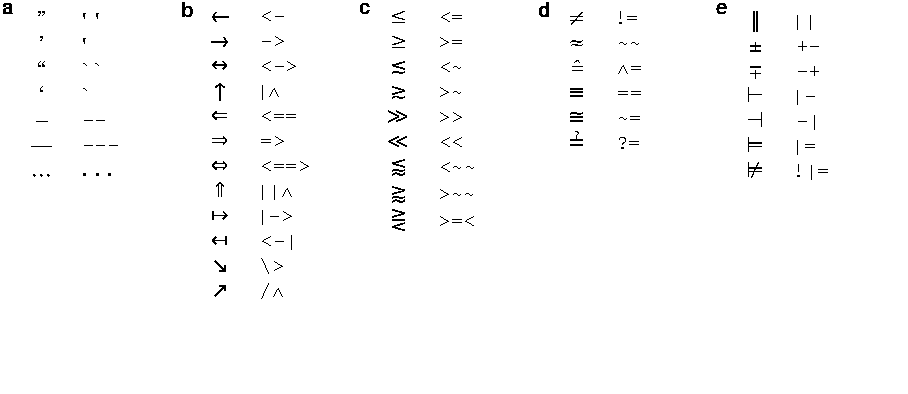
\includegraphics[scale=.85]{../doc/digraphs.pdf}\hfill~\vspace{-40pt}

\caption{{\bf Automatic character substitutions.} To get the glyph on
  the left, type the character sequence on the right. {\bf a.}~General
  punctuation. {\bf b.}~Arrows (see also Figure~\ref{fig:texcodes}i). {\bf c.}~Less than and greater
  than. {\bf d.} Decorated equals signs. {\bf e.}~Other mathematical
  operators.}\label{fig:charsubst}
\end{figure}

In addition to the automatic substitutions, there are many symbols
that can be obtained by typing a backslash followed by their name
(Figure~\ref{fig:texcodes}).  Extending this list
is easy, so let me know if you have suggestions.

As an alternative to standard unicode input methods for entering
accented letters, ELN supports creating a select group of accented
letters by typing a backslash followed by a symbol and a letter
(Figure~\ref{fig:accents}), as in ``{\tt Se\char92\char126nor}'' for
``Se\~nor'' or ``{\tt soup\char92,con}'' for ``soup\c{c}on''. 

\begin{figure}
\noindent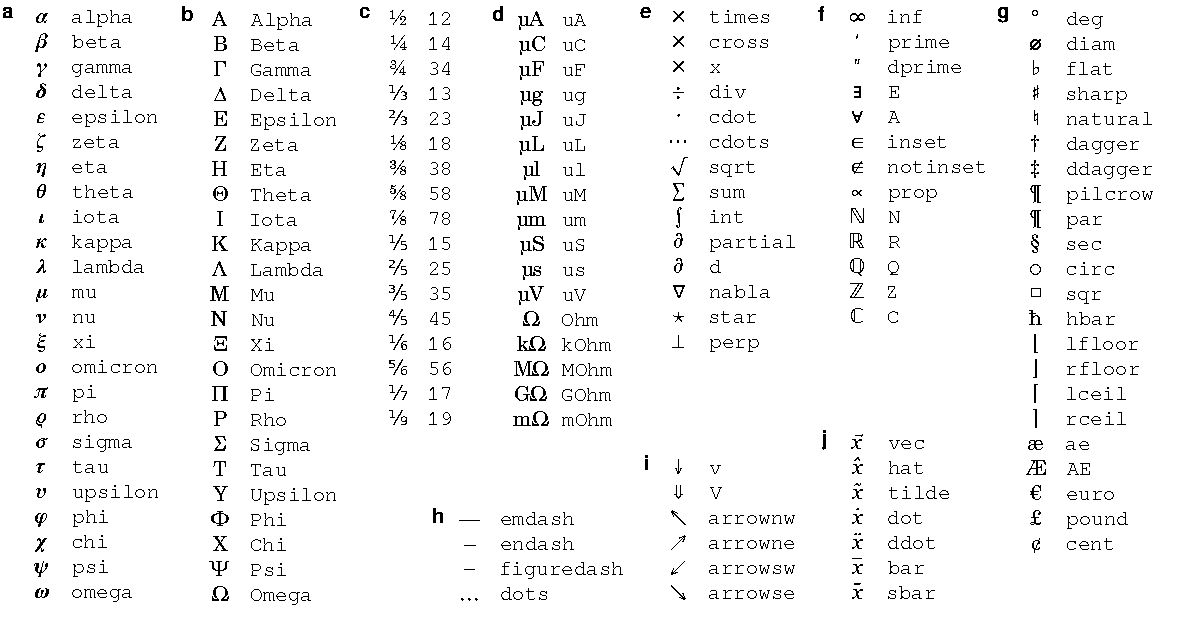
\includegraphics[width=\textwidth]{../doc/texcodes.pdf}\vspace{-7pt}

\caption{{\bf Symbols that may be obtained by a TeX-like command.} To
  get the symbols on the left, type a backslash followed by the character sequence on the
  right, then keep typing.
  {\bf a,~b.}~Lowercase and uppercase Greek letters.
  {\bf c.}~Fractions.
  {\bf d.}~Scientific units.
  {\bf e.}~Mathematical operators.
 {\bf f.}~Other mathematical symbols.
  {\bf g.}~Other symbols.
  {\bf h.}~General punctuation.
  {\bf i.}~Arrows.
  {\bf j.}~Mathematical accents.
  (The codes in \emph{j} are
  different from the others, in that the accent is placed over the
  preceding character rather than as a separate
  entity.)}\label{fig:texcodes}
\end{figure}

\begin{figure}
\noindent~\hfill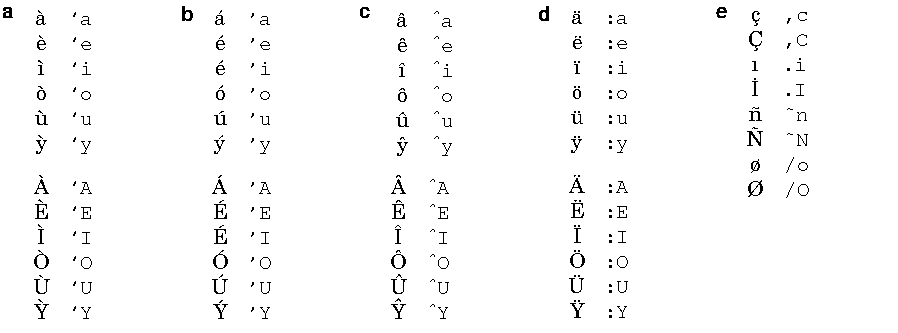
\includegraphics[scale=.85]{../doc/accents.pdf}\vspace{-7pt}\hfill~

\caption{{\bf Accented letters that may be obtained by a TeX-like sequence.} To
  get the accented letters on the left, type a backslash followed by the character sequence on the
  right, then keep typing.}\label{fig:accents}
\end{figure}


\section{Footnotes}

Press \keycontrol{N} to create a footnote. Footnotes are connected to
the main text by arbitrary tags: the word at the cursor becomes the
tag.  If you prefer to use symbols to tag footnotes, the symbols *,
\dag, \ddag, \S, \P, and $\sharp$ can be created by typing {\tt *},
    {\tt +}, {\tt ++}, {\tt\$}, {\tt @}, and {\tt \#} before pressing
    \keycontrol{N}. Footnotes are deleted by deleting the tag in the
    main text or by pressing \controlshift{N} while the tag is
    highlighted.

If your tag is a big integer, it is interpreted as a PubMed ID. In
that case, ELN will insert the corresponding citation in the note for
you automatically. (If you have suggestions for other kinds of
automatically created note contents, I want to hear from you.)

\section{Hyperlinks}

Press \keycontrol{L} to create a hyperlink. (If your hyperlink
contains spaces, you will have to select the text first, otherwise,
ELN figures out the boundaries of the link text automatically.)

Hovering over a link displays a thumbnail of the
page\footnote{Currently, the Mac and Windows versions merely show the
  title of a web page while hovering. I hope to restore thumbnailing
  when Qt's QWebEngine technology further matures.}, and double
clicking opens a pdf of the downloaded page. Double clicking with
\key{Shift} held opens the original web page. Hyperlinks are typeset
with a pale blue background once download is complete and with a pink
background if download fails. (A yellow background indicates that
download is in progress.)

\section{Magic links}

ELN recognizes not just URL-style hyperlinks, but also a number of
other ``magic'' links:
\begin{itemize}
\item A small number (at most 4 digits), upon pressing \keycontrol{L}
becomes a hyperlink to another page in the notebook.
\item A large number (more than 4 digits)
will be interpreted as a PubMed ID and will link to PubMed. When
possible, the corresponding article will be automatically downloaded
and archived with the notebook. 
\end{itemize}

\section{Typesetting quotations, computer code, and other imported materials}

Occasionally it is useful to typeset ``imported'' materials such as
quotations differently from the rest of your notes. In a small
concession to typographic nicety, ELN does this for you if you press
\keycontrol{Tab}.  The paragraph will be typeset in a slightly
different color, a slightly smaller point size, and with slightly
larger margins. To undo, simply press \keycontrol{Tab}
again. Similarly, indentation can be cycled between indented
paragraphs (the default), non-indented paragraphs, and ``dedented''
paragraphs, which is useful for typing bullet lists. This is done by
pressing \keyshift{Tab}.

\section{Typesetting mathematics}

When typing mathematical equations, having to frequently type the backslash for special characters and \keycontrol{/} for
italics can get tiresome. To avoid this annoyance, press
\keycontrol{`} (that's the key to the left of the \key{1} on many
qwerty keyboards) to enter (and exit) ``math'' mode, which turns the
\icon{type} icon into \icon{type-math}. (Math code can
also be entered by double-clicking the \icon{type} icon
or pressing \keyshift{F2}.)

In math mode, special characters can be entered simply by typing their
name and single-character words are typeset in italics.\footnote{A few
  exceptions apply: ``x'' does not generate $\times$, ``d'' does not
  generate $\partial,$ and ELN tries to guess whether you mean the
  variables $a$ and $I$ or the words ``a'' and ``I.'' A few other
  subtle cases are handled semi-intelligently as well.} Additionally,
simple subscripts and superscripts can be typeset by just typing
underscore or hat followed by the text of the sub- or superscript. As
a result, an equation like ``$\int_1^\infty 1/x^2\, \mathrm{d}x =
1$'' can be typeset simply by typing ``{\tt{int\char95{}1\char94inf
    1/x\char94{}2 dx = 1}}''. Even double superscripts and subscripts are possible,
to the degree that the second level is supported by
unicode.\footnote{At the moment, only single digits are
  supported. Outside of mathmode these can be obtained by typing
  ``{\tt \char92\char94{}2}'', ``{\tt \char92\char95{}2}'', etc.} For
instance, ``$\mathrm{e}^{-\sfrac12(x_1{}^2+x_2{}^2)}$'' can be typeset simply by
typing
``{\tt{e\char94\char123-\char92{}12(x\char95{}1\char94{}2+x\char95{}2\char94{}2)\char125}}''. (Note
how the curly braces ``protect'' the inner expression.)

\section{Typesetting computer code}\label{sec:codemode}

When typing computer code, the automatic substitions in
Figure~\ref{fig:charsubst}, \ref{fig:texcodes}, and~\ref{fig:accents} can be a
hindrance. To disable all automatic substitions, press \keycontrol{F2}
(or click the \icon{type} icon with \key{Ctrl} held). The icon will
change to \icon{type-code}, which signifies ``Code'' mode. Press
\key{F2} to return to normal text mode.

\section{Exporting and printing}

ELN can export your entire notebook or portions of it to pdf or print
them directly. Simply press \keycontrol{P} or click the
\icon{nav-print} icon
to open the print dialog and select either ``Print to pdf'' or an
actual printer.

Individual entries can also be exported as html by pressing
\controlshift{S}. This feature is still slightly experimental. Styling
is not yet quite how I would like it to be. In the future, html output
will likely be integrated with the print dialog. 

\section{Searching your notebook}

ELN incorporates a simple but very useful full-text search
facility. Press \keycontrol{F} or click the \icon{nav-find} icon to open the
search dialog, type any word or phrase, and press \key{Enter} or click
``OK.'' A list with search results from the entire notebook will open;
click on a result to navigate to the relevant entry.

\section{Customization}

At present, you cannot graphically change the looks of a
notebook. However, inside each notebook folder, ELN creates a file
called ``style.json'' that defines many of the style parameters of the
notebook. I don't have the time right now to document all of them
(feel free to contribute). Particularly important ones are
``page-width'' and ``page-height'' which specify the width and height
of a notebook page in points (1/72'') and the various
``\ldots-font-family'' variables.

\section{Archiving (version control)}

If you have Git installed on your computer, you can choose to have
your notebooks archived locally or to another computer using
Git. Simple enable the ``Archiving'' option and specify the place
where you want the archive to be stored.

Archiving locally is extremely easy, but of limited
utility.\footnote{Unless ``locally'' actually means a network location
  that your computer maps to a path that merely ``looks'' local to
  ELN.  Most operating systems are capable of that.} Archiving
remotely from within ELN is slightly more involved. If you have no
experience with Git, it is probably best to remedy that first. Some of
the following is likely to be hard to understand otherwise.

\emph{Caution: Black diamond contents ahead.} For remote archiving,
you need to have a host computer that you can access by ssh without a
password. Typically, that involves setting up a public/private RSA key
pair using ssh-keygen or similar and appending the public key to the
file ``.ssh/authorized\_keys'' on the server. Further details can be
found elsewhere. In my experience, doing this from a Windows computer
is much trickier than from either Linux or Mac OS; the most
workable Windows solution I have found is ``Pageant,'' which is part
of the ``PuTTY'' package.\footnote{At https://www.putty.org. See
  https://documentation.help/PuTTY/pageant.html for an introduction to
  Pageant.}

If you use Git to store your notebook on a remote host,
you can also access it from other computers. To do that, you would
select ``Clone hosted notebook for local use'' from the ELN opening
screen. Conveniently, once you have cloned the notebook, you can treat
it just like any other local notebook, with one caveat: you should not
open a notebook simultaneously on two computers, and always allow Git
to ``commit and push'' any changes back to the host.\footnote{If you fail to
heed this warning, ELN will likely have to manually rebuild your index
and table of contents. That's not the end of the world. However, in
rare instances, your notebook can get into a messy state from which
recovery will require typing Git commands in a terminal window. Note
that it is always completely safe to only use one client computer with
Git at a time.} Similar cautions apply when you use solutions like
Dropbox or iCloud for holding your notebook.

\emph{Warning: Double black diamond contents ahead.} It is also
possible to turn an existing notebook into a Git repository. There are
two steps:
\begin{enumerate}
  \item you should replace the line in your notebook's
    ``style.json'' file that says ``{\tt"vc":~""}'' to ``{\tt"vc":~"git"}'';
    \item you
should locate the ``.nb'' folder, type \terminal{git init} to turn your
notebook into a Git repository, then type some variant of

\terminal{ssh
\emph{user}@\emph{host} git init --bare
\emph{somewhere}/\emph{nice}/\emph{notebook}.nb}\vspace{-5pt}

\terminal{git push -u
\emph{user}@\emph{host}:\emph{somewhere}/\emph{nice}/\emph{notebook}.nb}

to set up the archive host.
\end{enumerate}
Again, if this section doesn't make sense to you, please first learn
about Git version control, then read it again before
contacting me. (And yes, I will be happy to assist.)

\section{Conclusion}

I hope that ELN will be useful to you, and that it will encourage you
to take more---and more usable---notes. I love to hear happy users'
stories. I also welcome bug reports of all kinds. And in the unlikely
event that ELN appears to have chewed up your notes, please do not
just throw away the broken notebook. Although I cannot make any
guarantees (see the GPL license text!), it almost certainly can be
fixed. And I would be happy to try and help.

\bigskip

\noindent Pasadena, May 2013;

\noindent Cincinnati, February 2014;

\noindent Woods Hole, June 2015;

\noindent Pasadena, January 2016, January 2017, April 2019;

\noindent Altadena, November 2020.

\end{document}
